\documentclass[aspectratio=169]{beamer}
\usepackage{CustomTheme}

\addbibresource{cv-for-ch/01-HTR.bib}

\newfontfamily{\junicodeFont}{Junicode-Regular.ttf}
\newcommand{\juni}[1]{{\junicodeFont #1}}
\newcommand{\character}[1]{{‹#1›}}
\newcommand{\mss}[1]{\textit{#1}}

\title[CV 4 CH]{Handwritten Text Recognition}\subtitle{Usability, Reusability and Exploitations}
\date[2024]{Computer Vision for CH}
\begin{document}

%The next statement creates the title page.
\frame{\titlepage}

\begin{frame}{The course}
    \begin{itemize}
        \item Week 1, Handwritten Text Recognition
        \item Week 2, Session 1, (Malamatenia Vlachou-Efstathiou) Digital Palaeography
        \item Week 2, Session 2, Distant Viewing
    \end{itemize}
\end{frame}

\section{Introduction}

\begin{frame}{HTR or HTR Workflows ?}
    \begin{minipage}{.45\textwidth}
        \begin{enumerate}
            \item<1-> A Picture
            \item<2-> (Opt.) Post-processed
            \item<3-> Layout Analysis (Zones \& Lines)
            \item<4-> Text Prediction ($\leftarrow \text{HTR}$)
            \item<5-> (Opt.) Manual Correction
            \item<6-> Data Retrieval
            \item<6-> Project workflow... 
        \end{enumerate} 
    \end{minipage} \hfill
    \begin{minipage}{.45\textwidth}
        \begin{figure}
            \centering
            \includegraphics<1>[width=.8\linewidth]{cv-for-ch/images/ManuscriptExample.png}
            \includegraphics<2>[width=.8\linewidth]{cv-for-ch/images/ManuscriptEnhanced.png}
            \includegraphics<3>[width=.8\linewidth]{cv-for-ch/images/ManuscriptSegmented.png}
            \includegraphics<4>[width=.8\linewidth]{cv-for-ch/images/ManuscriptTranscribed.png}
            \includegraphics<5>[width=.8\linewidth]{cv-for-ch/images/ManuscriptCorrected.png}
            \includegraphics<6>[width=.8\linewidth]{cv-for-ch/images/ManuscriptExported.png}
        \end{figure}
    \end{minipage}
\end{frame}

\begin{frame}{Artificial Intelligence?}
    \begin{minipage}{.65\textwidth}
        In the context of ATR, AI = 
        \begin{itemize}
            \item Algorithms (model architectures)
            \item Software (Implementation of architectures)
            \item Models (Weights learned by the model)
            \item Training data
        \end{itemize}
        But also very often:
        \begin{itemize}
            \item Infrastructure or computing hardware (GPU for training, CPU for inference)
            \item Infrastructure for data creation
            \item Research!
        \end{itemize}
    \end{minipage} \hfill
    \begin{minipage}{.30\textwidth}
        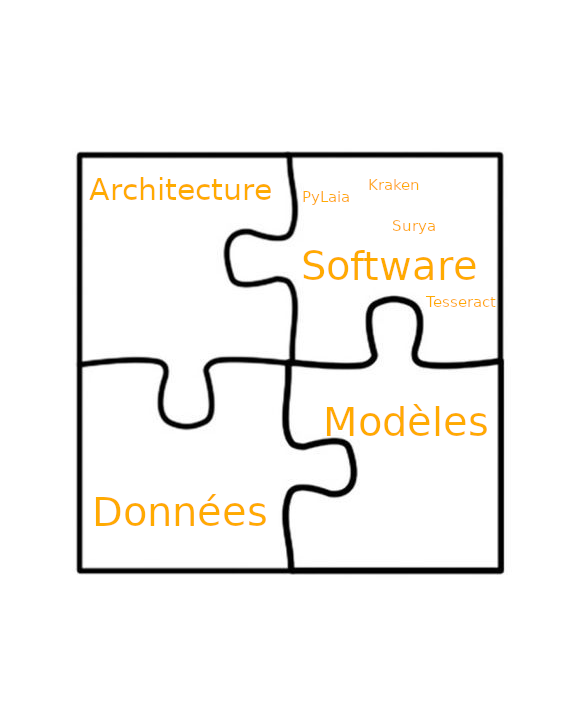
\includegraphics[width=\linewidth]{cv-for-ch/images/PuzzleATR.png}
    \end{minipage}
\end{frame}

\begin{frame}{HTR: Baseline vs. BBoxes}
    Two HTR paradigms:
    \begin{itemize}
        \item HTR Engine based on baseline (through segmentation) that uncurves baselines and computes polygons around the line. That's what Kraken does. This allows for the handling of curved and round lines. Allows for more exotic situations.
        \item HTR Engine based on BBox or complex polygon: a rectangle is drawn around the text, leaving potential noise of the previous and next lines inside. Unable to deal with curved lines.
    \end{itemize}
    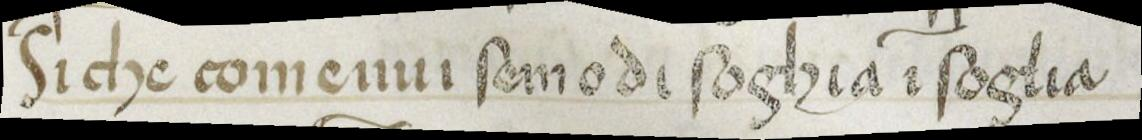
\includegraphics[width=.4\linewidth]{cv-for-ch/images/htr-polygons.jpg}\hfill
    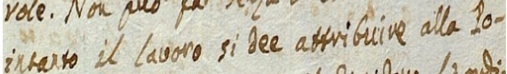
\includegraphics[width=.4\linewidth]{cv-for-ch/images/htr-bbox.png}
\end{frame}

\begin{frame}{A revolution in the OCR world ?}
    \begin{columns}
        \begin{column}{.4\linewidth}
            More and more transformer-based architecture meant to do everything at once: segmentation, text recognition and formatting. For example, the Nougat model from Meta\footfullcite{blecher2023nougatneuralopticalunderstanding}.
        \end{column}
        \begin{column}{.6\linewidth}
            \vspace{.3em}
            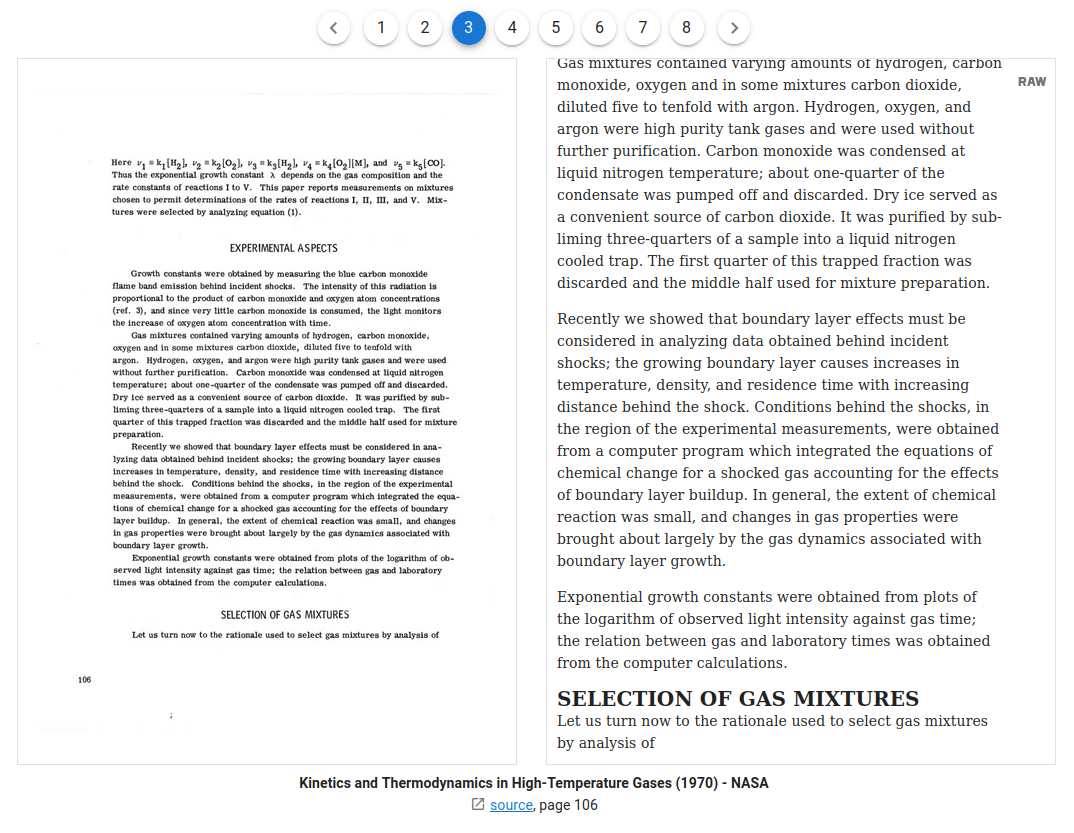
\includegraphics[width=\linewidth]{cv-for-ch/images/htr-nougat.png}
        \end{column}
    \end{columns}
    \centering
\end{frame}

\begin{frame}{The notion of Generic Models}
    \only<1-4>{
        \begin{itemize}
            \item<1-> Generic Models are models thought to be compatible with a wide variety of documents, in a specified space: generic can be ultra-generic (any kind of script, any period) or generic within a smaller space (any Latin mss 10 to 12th cent)
            \item<2-> Generic Models aim at balancing overall accuracy on all documents rather than learning more about a single one.
            \item<3-> Specific Models are generally either created from scratch (trained from data of a specific manuscript or subset of), or derived from a generic model: we take the weight of a generic model and further teaches it to learn more about a new subset of documents.
            \item<4-> This Generic $\rightarrow$ Specific Models process is called fine-tuning, and it allows for faster training time (less energy, less money spent) but also in the case of small dataset better result: the model does not start from kindergarten again, and can keep some of its previous knowledge as well.
        \end{itemize}
    }
    \centering
    \includegraphics<5>[width=.8\linewidth]{cv-for-ch/images/htr-General.jpg}
\end{frame}

% \begin{frame}{Papers}

% \fullcite{clerice2024catmus}

% \vspace{1em}

% \fullcite{wauchier2019}
    
% \end{frame}

\section{Issues that require solutions}

\begin{frame}{HTR and Medieval Time Issues}
    \only<1->{
        \begin{figure}
            \centering
            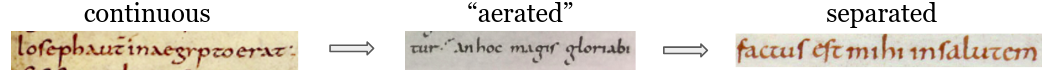
\includegraphics[width=\linewidth]{cv-for-ch/images/htr-spacing.png}
            \caption{Spacing}
        \end{figure}
    }
    \begin{columns}
        \begin{column}{.5\linewidth}
            \only<2->{
                \begin{figure}[h]
                    \centering
                    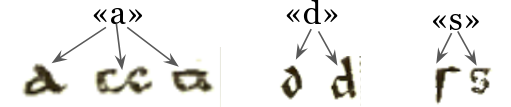
\includegraphics[width=\linewidth]{cv-for-ch/images/htr-allographs.png}
                    \caption{Allographs}
                \end{figure}
            }
        \end{column}
        \begin{column}{.5\linewidth}
            \only<3->{
                \begin{figure}[h]
                    \centering
                    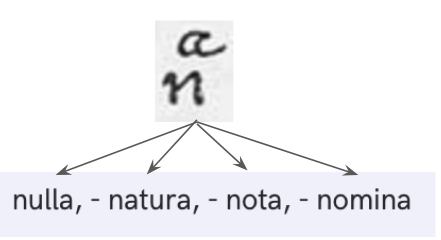
\includegraphics[width=.8\linewidth]{cv-for-ch/images/htr-abbreviation.png}
                    \caption{Abbreviations}
                \end{figure}
            }
        \end{column}
    \end{columns}
\end{frame}

\begin{frame}{Graphical Variations}
    \begin{figure}
        \centering
        \includegraphics<1>[width=\linewidth]{cv-for-ch/images/Scripts.png}
        \includegraphics<2>[width=\linewidth]{cv-for-ch/images/Diversity.png}
    \end{figure}
    
    \only<1>{A (small) sample of the types of scripts that can be found...}
    \only<2>{and their manifestations!}
\end{frame}
\begin{frame}{What is transcription?}

\begin{minipage}{.45\textwidth}
    Transcribing is: 
    \begin{itemize}
        \item Making choices;
        \item Interpreting;
        \item Translating;
        \item Describing.
        \note{Semantic, visual, and usability compromises};
    \end{itemize} 
    Transcribing is therefore betraying.
\end{minipage}\hfill
\begin{minipage}{.35\textwidth}
    \centering
    \vspace{1em}
    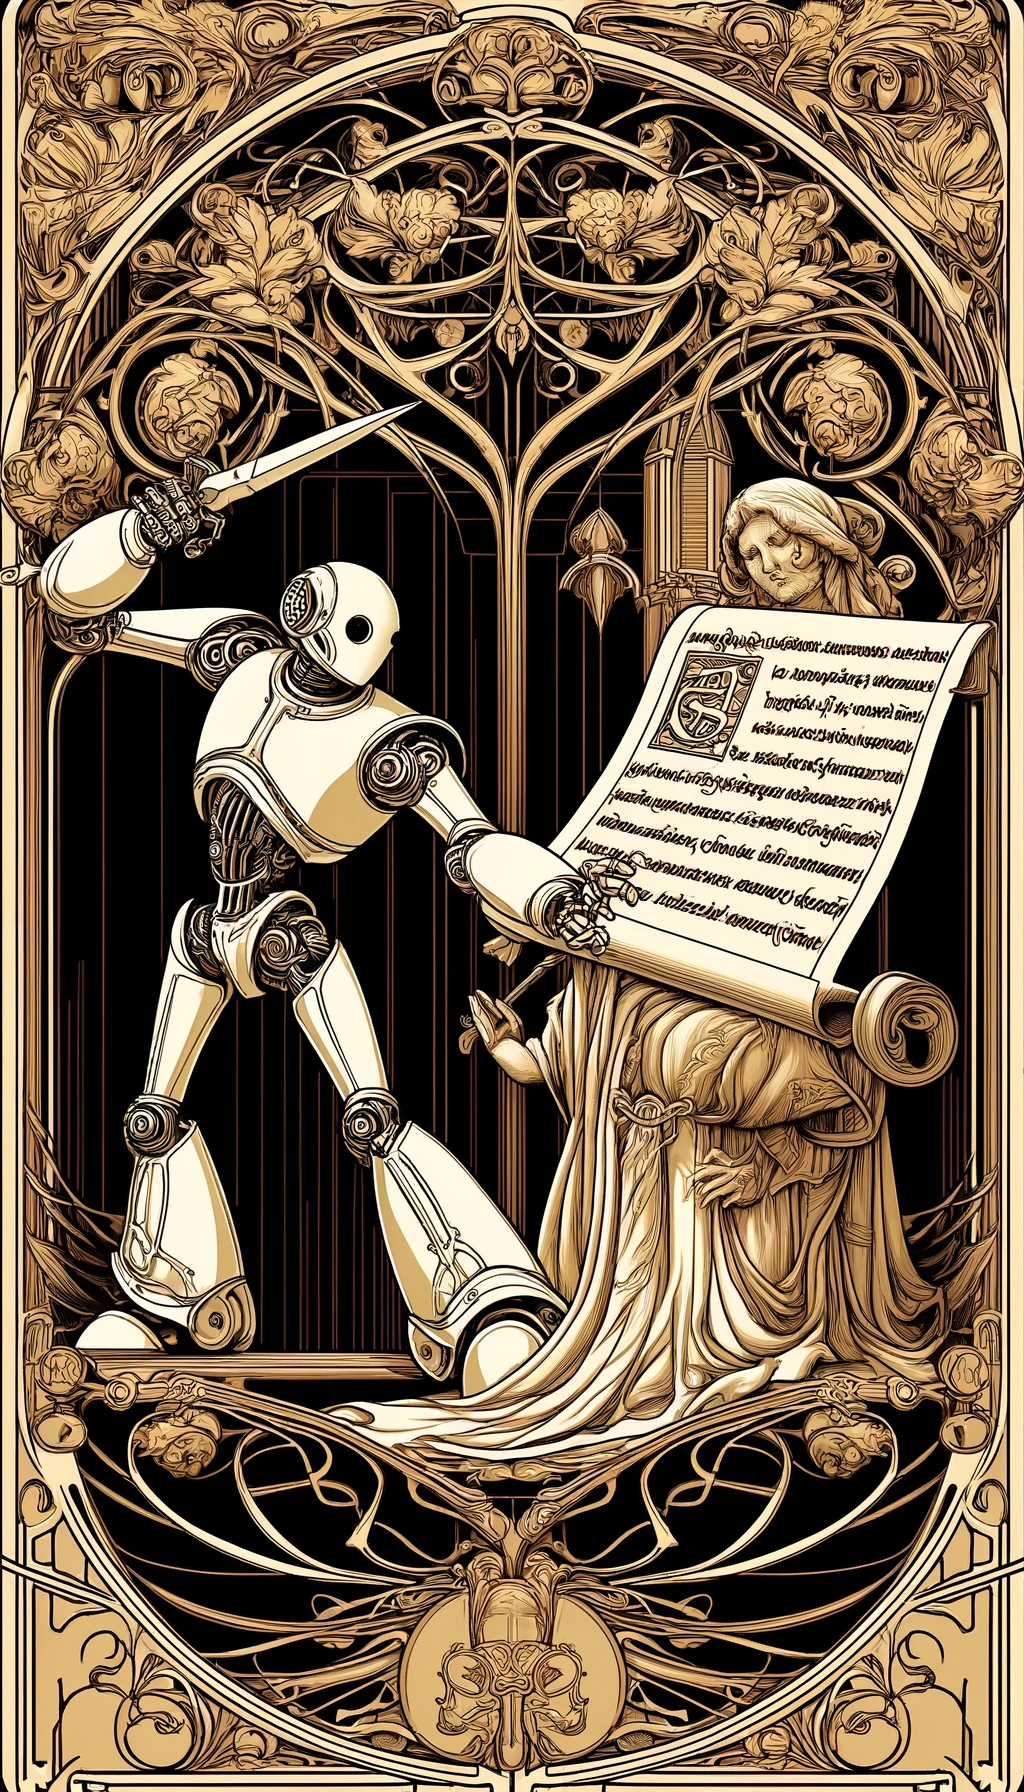
\includegraphics[width=.8\linewidth]{cv-for-ch/images/Trahir.png}
\end{minipage}

\end{frame}

\begin{frame}{The choices}
    \begin{minipage}{.45\textwidth}
        \begin{enumerate}
            \item<1-> What are the different transcription questions?
            \item<2-> Textual content (Abbreviation/Normalization)\only<2>{: should we write Charles (as in a book), Carles (without homogenization), Carl̃. (Unresolved abbreviation), carł. (Preserving the forms)}
            \item<3-> Punctuation (Modernization/Reproduction)\only<3>{: \enquote{,} (modernized), \enquote{.} ("semantic"), \enquote{·} (faithful to the manuscript?)}
            \item<4-> Graphical variation of letters\only<4>{: round s or long s?}
            \item<5-> Spacing issues\only<5>{: \enquote{ma tere} (modern)? \enquote{matere} (presence/absence)? \enquote{m a tere} (proportional)?}
        \end{enumerate} 
    \end{minipage} \hfill
    \begin{minipage}{.32\textwidth}
        \begin{figure}
            \centering
            \vspace{1em}
            \includegraphics<1>[width=1\linewidth]{cv-for-ch/images/ExempleBase.jpg}
            \includegraphics<2>[width=1\linewidth]{cv-for-ch/images/ExempleAbrev.jpg}
            \includegraphics<3>[width=1\linewidth]{cv-for-ch/images/ExemplePonctuation.jpg}
            \includegraphics<4>[width=1\linewidth]{cv-for-ch/images/ExempleAllographe.jpg}
            \includegraphics<5>[width=1\linewidth]{cv-for-ch/images/ExempleSegmentation.jpg}
        \end{figure}
    \end{minipage}
\end{frame}

\section{Transcription Guidelines ?}

\begin{frame}[t]{Producing refinable and reusable data}
    \vspace{1em}
    \begin{columns}
        \begin{column}{.45\textwidth}
            There are three options: \note{State that this is also according to the goals of a project}
            \begin{enumerate}
                \item<1-> Allograph transcription\only<1>{
                    \begin{itemize}
                        \item One handwritten sign = one digital sign.
                        \item Unit: allograph.
                        \item Reduced language model.
                        \item Large number of classes.
                        \item Rare classes = no recognition.
                        \item Risk of missing Unicode symbols!
                        \item The more classes, the higher the error rate.
                    \end{itemize}
                }
                \item<2-> \enquote{Edition-style} transcription\only<2-3>{
                    \begin{itemize}
                        \item Unit: word
                        \item Resolution of abbreviations,
                        \item Punctuation normalization according to modern practices,
                        \item More easily exploitable data,
                        \item "Cheaper" in the short term\note{possible alignments!};
                        \item<3> \textbf{BUT} the machine sees only one line at a time,
                        \item<3> Context is sometimes insufficient!
                        \item<3> Depends on the language, document, and genre!
                    \end{itemize}
                }
                \item<4-> Graphematic transcription\only<4>{
                    \begin{itemize}
                        \item One handwritten sign = one digital sign.
                        \item Unit: character\note{Many-to-one mapping}
                        \item Preservation of abbreviations
                        \item Compromise between simplifying ML tasks and usability
                        \item More independent from linguistic variations
                        \item \textbf{But} requires post-processing
                    \end{itemize}
                }
            \end{enumerate}
            \only<5>{Only the first option can automatically convert into the third.}
            \only<5>{
                \begin{itemize}
                    \item $v \rightarrow u$, $j \rightarrow u$ and similar are easy to do.
                \end{itemize}
            }
        \end{column} 
        \hfill
        \begin{column}{.40\textwidth}
                \centering
                \includegraphics<1>[trim={0 9.5cm 0 10cm},clip,width=1\linewidth]{cv-for-ch/images/AllographeticDebates.png}
                \includegraphics<2>[trim={0 4em 0 2em},clip,width=.8\linewidth]{cv-for-ch/images/ApprocheEditoriale.png}
                \includegraphics<4>[width=1\linewidth]{cv-for-ch/images/Capelli.png}
                \only<4>{Cappelli, “The Elements of Abbreviation”, p. 13}
        \end{column}
    \end{columns}
\end{frame}

\section{So what if I go the editorial way ?}

\begin{frame}{A model is just as clever as its data}
    \begin{itemize}
        \item A model is produced on data. \textbf{It learns what it sees}.
        \item A (Kraken) model \textbf{sees line by line}, it's the only context it has.
        \item A (Kraken) model does \textbf{learn some languages features by "accident"} when being trained. And the \textbf{more} a dataset is \textbf{multilingual} or include linguistic differences (lexical, spelling, syntax to a certain degree), the \textbf{more} it \textbf{resists} guessing based on linguistic features.
        \item As a consequence, a (Kraken) model \textbf{trained on one language} only will always \textbf{perform poorly on another language}, or to be precise, more poorly than if it had been trained on the second one: \textbf{models are lazy, they take the easy path.}
        \item You can teach a model to normalize text. But then, what am I teaching and asking from the model ? Am I giving the model as much knowledge as the editor has when they read (paratextual knowledge specifically) ?
        \item<2> \textbf{And if I do, because it's more convenient, what do I risk ?}
    \end{itemize}
\end{frame}

\begin{frame}{e-NDP Model}
    \only<1>{
        \begin{columns}
            \begin{column}{.7\linewidth}
                \fullcite{jdmdh:12732}
            \end{column}
            \begin{column}{.3\linewidth}
                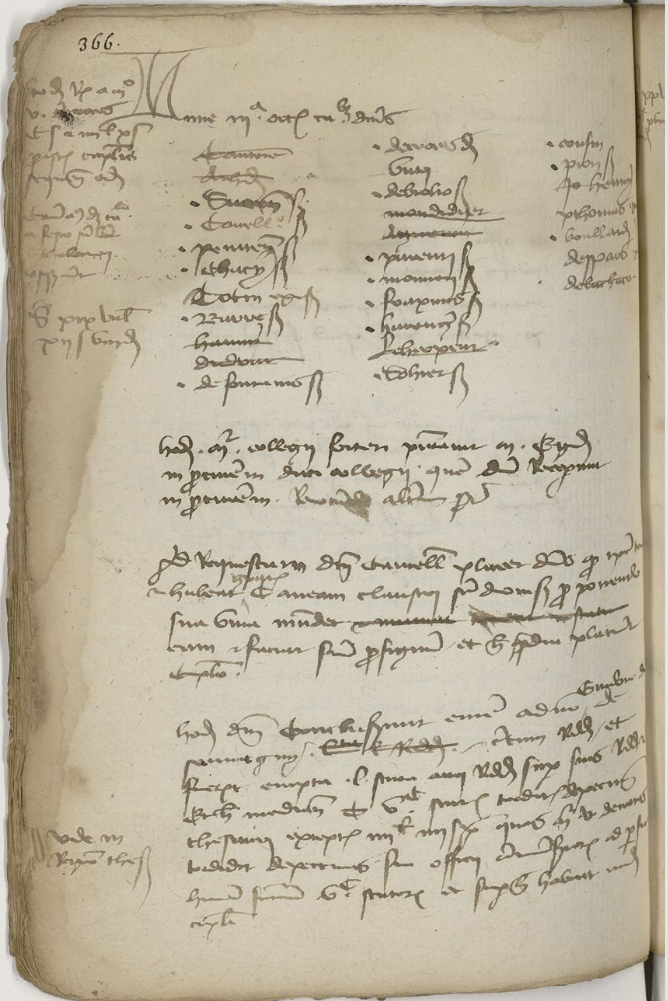
\includegraphics[width=\linewidth]{cv-for-ch/images/endp.png}
            \end{column}
        \end{columns}
    }
    \only<2>{
        \enquote{\footnotesize
            \textit{Upon closer examination, these errors often coincide with misrecognition of typical phenomena in medieval handwriting. These include indistinctness in characters composed of successive minims (single strokes), such as n, m, i, u (e.g., indiuidue, mandauimus); misrecognized ligatures, such as st and ct; \textbf{undeveloped or incompletely developed abbreviations by suspension}, which are easy to fit (e.g., no[-bis], franc[-orum]); \textbf{by contraction}, which are harder to fit (e.g., m[a]g[is]t[er], d[o]m[i]n[us]); abbreviations whose \textbf{expansion depends on the declension}, (v.g. ‘Par.’ which can be resolved as Par[is], Par[isiensis] or Par[isiense] depending on the context)}.
        }
        \cite{jdmdh:12732}
    }
    \only<3>{Example: \url{https://endp.chartes.psl.eu/facsimile/LL119/369}}
\end{frame}

\begin{frame}{Transformer model: bigger, better ?}
    \only<1>{
        \begin{columns}
            \begin{column}{.7\linewidth}
                \fullcite{aguilar2024handwritten}
            \end{column}
            \begin{column}{.3\linewidth}
                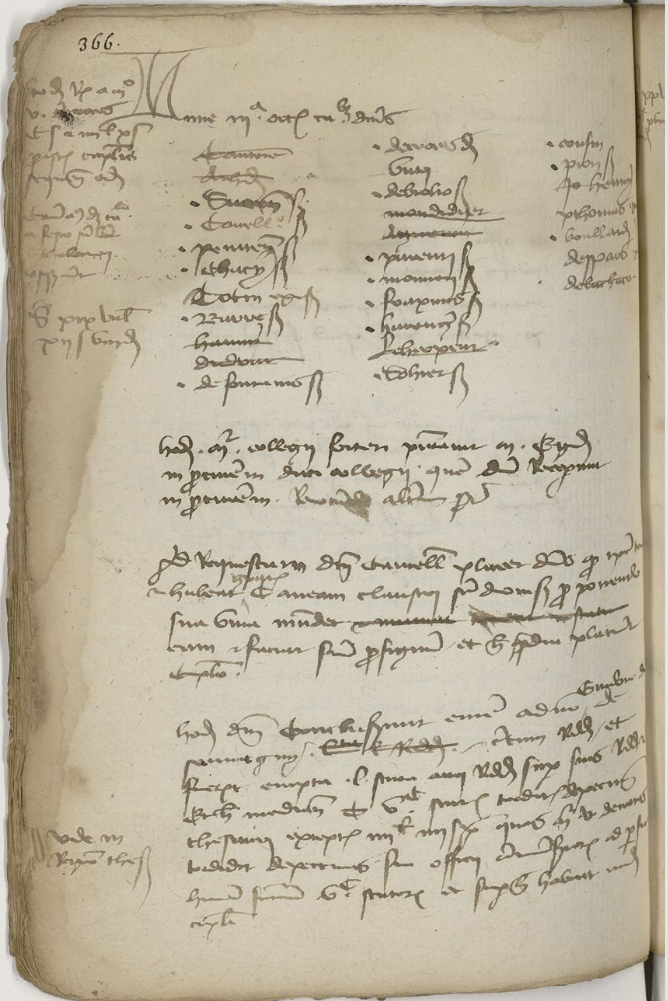
\includegraphics[width=\linewidth]{cv-for-ch/images/endp.png}
            \end{column}
        \end{columns}
    }
    \only<2>{
        \enquote{\footnotesize The efficacy of using explicit language models to improve the accuracy of HTR has been demonstrated in previous studies, yielding promising results[...]. These models capture statistical correlations among tokens in natural language, providing context awareness and proposing more contextually appropriate interpretations. This is particularly crucial for addressing challenges such as complex layouts, ancient or noisy writing, or\textbf{out-of-domain issues, where a purely graphical interpretation may fall short} in providing an accurate transcription, as it lacks the linguistic nuances and contextual understanding that language models bring to the table. In contrast to classical CRNN models, which implicitly learn language features and focus on identifying patterns directly from the data [...], the integration of a language model involves a statistical analyze of how words interrelate in a language and the likelihood of certain sequences co-occurring. This approach results in more precise and contextually informed predictions.}\cite{aguilar2024handwritten}
    }
    \only<3>{
        \enquote{\footnotesize Most errors from Transformer models are linked to mis-predictions at the word or sub-word level, paradoxically increasing the CER more than the WER. [...] This strategy is highly effective, as evidenced by the significant difference in WER between Transformer and CRNN models. CRNN models often propose seemingly verbatim transcriptions [..., that] “imitate” the input, especially when faced with unfamiliar words or phrases, rather than understanding the underlying linguistic patterns. Consequently, many of their outputs ignore the lexical relationships within the text, resulting in transcriptions that may be technically accurate at the character level but correspond to non-existent or nonsensical words.} \cite{aguilar2024handwritten}
    }
    \only<4>{
        \enquote{\footnotesize Most errors from Transformer models are linked to mis-predictions at the word or sub-word level, paradoxically increasing the CER more than the WER. [...] This strategy is highly effective, as evidenced by the significant difference in WER between Transformer and CRNN models. CRNN models often propose seemingly verbatim transcriptions [..., that] “imitate” the input, especially when faced with unfamiliar words or phrases, rather than understanding the underlying linguistic patterns. Consequently, many of their outputs ignore the lexical relationships within the text, resulting in transcriptions that may be technically accurate at the character level but correspond to non-existent or nonsensical words.} \cite{aguilar2024handwritten}
    }
    \only<5>{
        \centering
        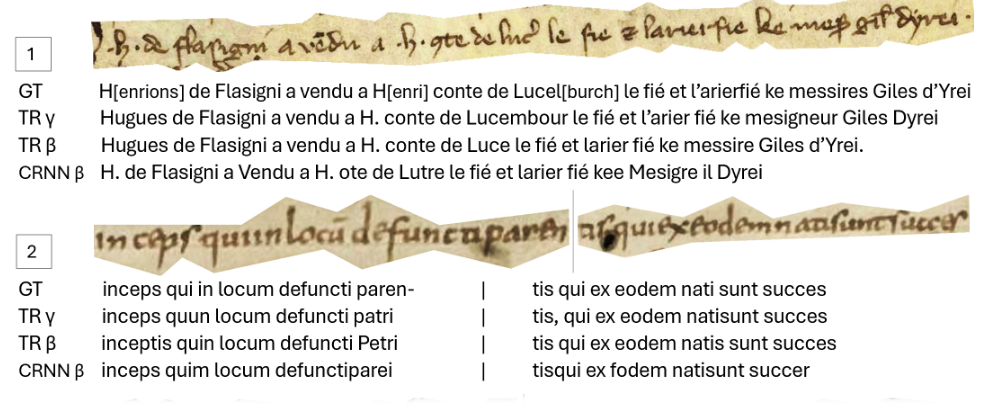
\includegraphics[]{cv-for-ch/images/aguilar-1.png}
    }
    \only<6>{
        \centering
        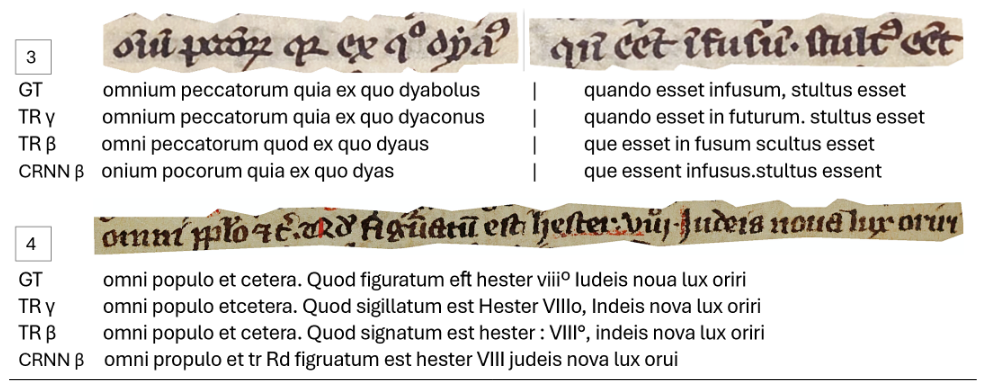
\includegraphics[]{cv-for-ch/images/aguilar-2.png}
        \vspace{1em}

        
        T. expanded to Tours instead of Trèves, because Trèves was not in the data: models are situated, constrained. Abbreviation expansion needs context.
    }
\end{frame}

\begin{frame}{And in other periods ?}
    \only<1>{
        \fullcite{normalizedvsdiplomatic}
    }
    \only<2>{
        \centering
        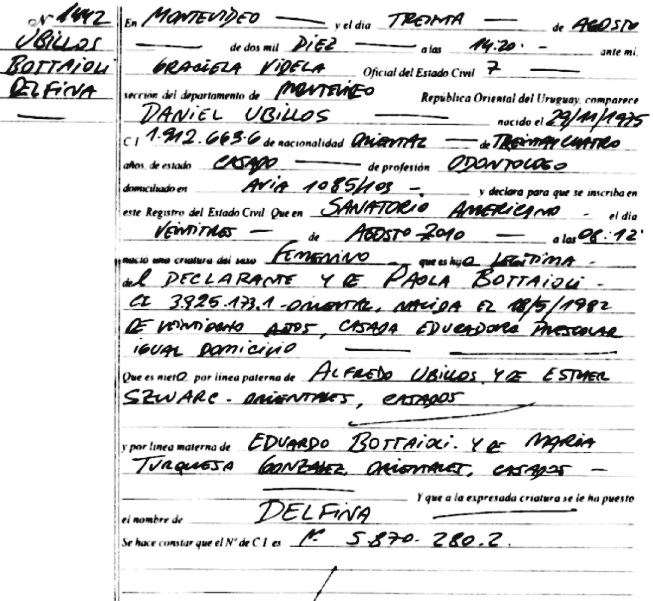
\includegraphics[width=.5\linewidth]{cv-for-ch/images/teklia-1.png}
    }
    \only<3>{
        \centering
        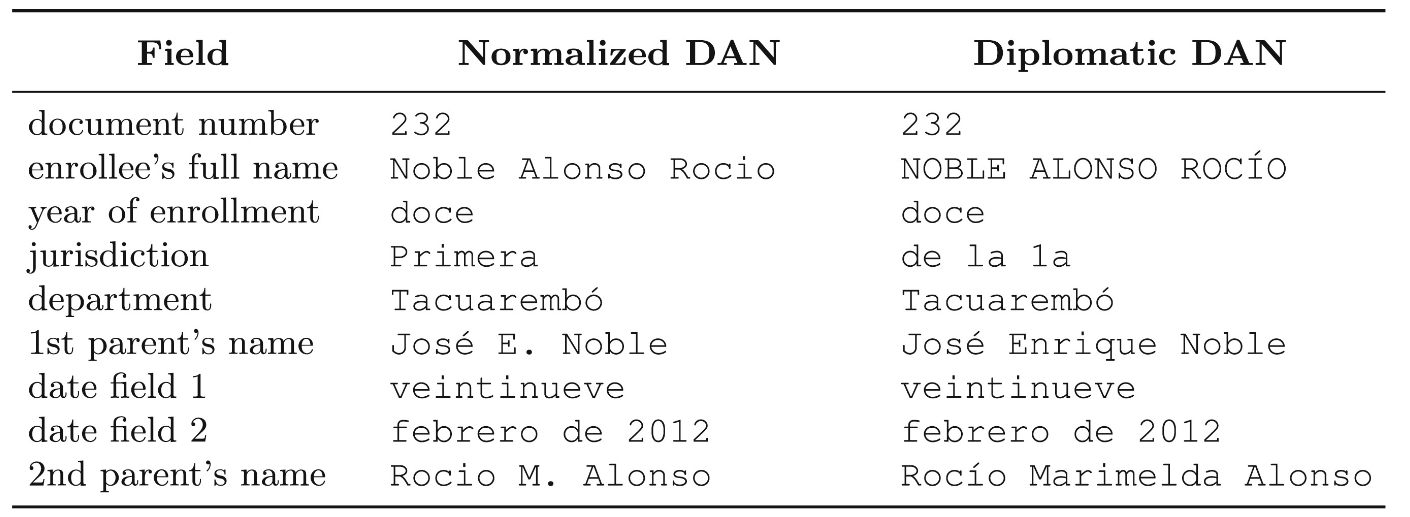
\includegraphics[width=.7\linewidth]{cv-for-ch/images/teklia-2.png}
    }
    \only<4>{
        \centering
        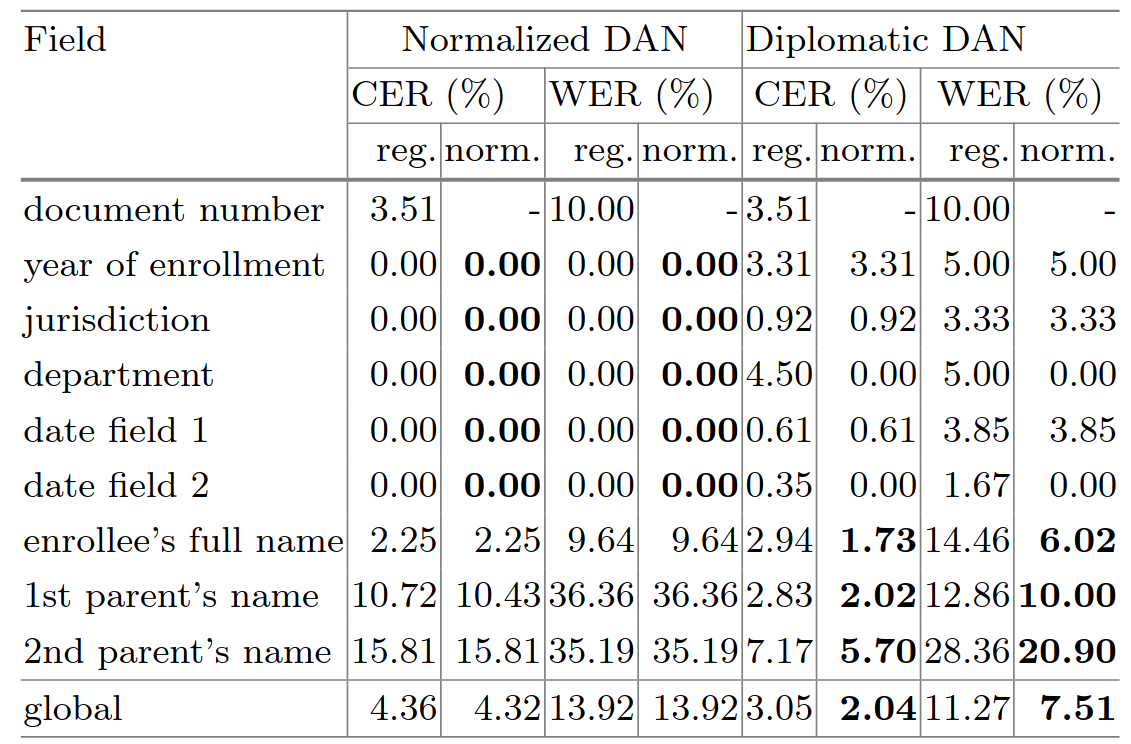
\includegraphics[width=.7\linewidth]{cv-for-ch/images/teklia-3.png}
    }
    \only<5>{
        \enquote{\footnotesize One of the possible reasons why Diplomatic DAN works better than Normalized DAN on these three fields was already explained in the description of the dataset: annotations provided by the civil registry included some abbreviation criteria on both parents’ names fields where, very frequently, the second name was abbreviated to its initial (e.g., “Alberto Carlos Bustos” was transcribed as “Alberto C. Bustos”). Somehow, this was learned by the model but with mixed results. In cases where the enrollee has a second name and the model was able to understand which letter to use, Normalized DAN produced a correct output (i.e. correctly abbreviated the middle name). In other cases, it made a mistake when abbreviating the middle name. \textbf{In cases where no middle name was handwritten in the document, the model just invented one}, presumably to agree with the format of the data it was trained on.} \cite{normalizedvsdiplomatic}
    }
\end{frame}

\begin{frame}{And finally, what are the consequences}
    \begin{itemize}
        \item There are very few combinations of fields (history, literature, philology, etc.), countries (France, Italy, Spain, Germany) or even subcategories (anglo-normand specialists vs. picard specialist) that would produce the same transcription depending on the tradition of their field.
        \item Any error is lost to the HTR: the decision to resolve is not visible in these models. The only reason these errors were caught is because papers' authors looked at the result.
        \item Punctuation, capitalization, normalization of abbreviation are domain-specific.
        \item<2> \textbf{This means that no datasets would be compatible !}
        \item<2> A solution is then to keep an approach that stay simple and leave some work for the researchers. And we can see how to address, domain per domain, what we can do to semi-automatize the translation.
    \end{itemize}
\end{frame}


\section{CATMuS Medieval}

\begin{frame}{Paper}
    \fullcite{clerice2024catmus}

    Also \url{https://catmus-guidelines.github.io} and \url{https://huggingface.co/datasets/CATMuS/medieval}
\end{frame}

\begin{frame}{Guidelines: Characters}
    \begin{itemize}
        \item Graphic distinctions for the same character like \character{s} (\enquote{round \character{s}}) and \character{ſ} (\enquote{long} \character{s}), or \character{\juni{ꝛ}} (\enquote{round} \character{r}) and \character{r} (\enquote{short} \character{r}), are disregarded to mitigate potential cascading effects on other letters like a, d, e, etc.
        \item Ligatures between letters, such as \character{st} or \character{ct}, are treated as variations in form, leading to the independent transcription of their constituent characters.
        \item Any emphasis on the letter, regardless of its form, is transcribed as capital letters, including if the emphasis is only conveyed by the size of the letter (and does not result in a different shape).
    \end{itemize}
\end{frame}

\begin{frame}{Guidelines: Abbreviation}
    The various signs fall into two main categories:
    \begin{enumerate}
        \item A large number are additions to base letters with diacritical marks, such as macrons (\textit{e.g.} \character{ē} for \textit{est}, \textit{-em}, etc.), and superscript letters (\character{q\textsuperscript{i}} for \textit{qui}), and their meaning is often context-dependent. Diacritics are thus treated as separate characters using Unicode decomposed form (NFD).
        \item Few are separate semantically distinct signs, such as \character{\&} for \textit{et/e}), or letters with strike-through marks, such as \character{\juni{ꝑ}}. For these, we resorted to the  Medieval Unicode Font Initiative (MUFI) \cite{mufi2009}.
    \end{enumerate}
\end{frame}

\begin{frame}{Guidelines: Ponctuation}
    \begin{itemize}
        \item Single full stops are transcribed as \character{.};
        \item Double signs are represented by \character{;};
        \item Commas are transcribed as \character{,},
        \item Question marks are transcribed as \character{?}, as soon as they appear in the Latin inventory in late middle ages.
    \end{itemize}
\end{frame}

\begin{frame}[shrink=10]{Datasets}
\vspace{1em}
    \begin{table}
    \centering
    \resizebox{.9\linewidth}{!}{
    \begin{tabular}{lcrccccccr}
        \toprule
Dataset                            & Type    & Century   & Language     & Script type   & Task         & Abbr. & Char.      & Modern.    & Quantity    \\ 
                                   &         &           &              &               &              &  Res. & Var.       &            &             \\ \hline
IAMHistDB/St. Gall                 & Mss     & 9         & Latin         & Bookscript    & HTR          &            &            &            & 1,410 l.    \\ 
IAMHistDB/Perzival                 & Mss     & 13        & German       & Bookscript    & HTR          & \checkmark & \checkmark &            & 4,477 l.    \\ 
ICFHR 2016-READ                    & Mss     & 15-19     & Ger.         & Modern        & HTR          &            &            &            & 10,550 l.   \\ 
ORIFLAMMS                          & Mss     & 12-14     & French, Lat. & Book., Docum. & HTR          & \checkmark & \checkmark & \checkmark & 120,111 l.  \\
HIMANIS                            & Mss     & 14-15     & Fr., Lat.    & Documentary   & HTR          & \checkmark & \checkmark & \checkmark & 23,112 l.   \\
HOME - Alcar                       & Mss     & 12-14     & Fr., Lat.    & Bookscripts   & HTR, NER     & \checkmark &            & \checkmark & 74806 l.    \\
e-NDP                              & Mss     & 14-16     & Fr., Lat.    & Documentary   & HTR          & \checkmark &            & \checkmark & 33,735 l.   \\ 
RODRIGO                            & Mss     & 16        & Spanish      & Bookscript    & HTR          &            &            &            & 20,357 l.   \\ 
Esposalles/INDEX                   & Mss     & 15        & Catalan      & Modern        & HTR          &            &            &            & 1,563 l.    \\ 
LAM                                & Mss     & 17-18     & Italian      & Modern        & HTR, DC      &            &            &            & 25,823 l.   \\ \midrule
MPS                                & Mss     & 13-16     & Dutch        & Documentary   & DC           &            &            &            & 1,706 d.    \\ 
CLAMM                              & Mss     & 5-15      & Lat.         & Bookscripts   & SC, DC       &            &            &            & 10,800 i.   \\ 
Multiple Font Groups & EP      & 15-17     & Multi.       & Fonts         & FC           &            &            &            & 35,623 i.   \\ \midrule
\only<2>{
CATMuS (Ours)             & Mss, EP & 8-16      & Multi.       & Bookscripts   & HTR, SC, DC  &            &            &            & 165,347 l.  \\
                                   &         &           &              & Documentary   &              &            &            &            &             \\
                                   &         &           &              & Fonts         &              &            &            &            &             \\ \bottomrule }
    \end{tabular}}
    \caption{Overview of parallel datasets. \textit{Abbr. Res.} = resolved abbreviations. \textit{Char. Var.} = allographetic \character{s}/\character{\juni{ſ}}). \textit{Modern.} = edition-like modernization. Mss stands for Manuscripts, EP for Early Prints, SC/FC/DC for Script, Font, and Date Classification.}
    \label{tab:concurrent_datasets}
\end{table}
\end{frame}

\begin{frame}{Dataset: Scripts}
    \begin{figure}[t]
        \centering
        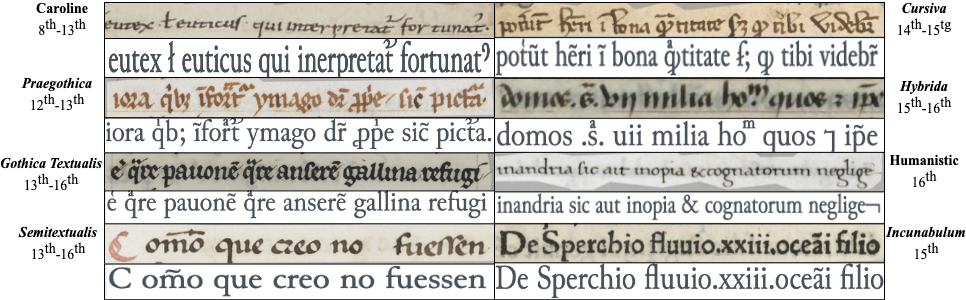
\includegraphics[width=\linewidth]{cv-for-ch/images/Scripts.png}
        \caption{Representative examples of the main script types lines, with CATMuS annotations.}
        \label{fig:script-reference}
    \end{figure}
    
\end{frame}

\begin{frame}{Dataset: Statistics}
    
    \begin{figure}[h]
      \begin{subfigure}[T]{0.40\textwidth}
        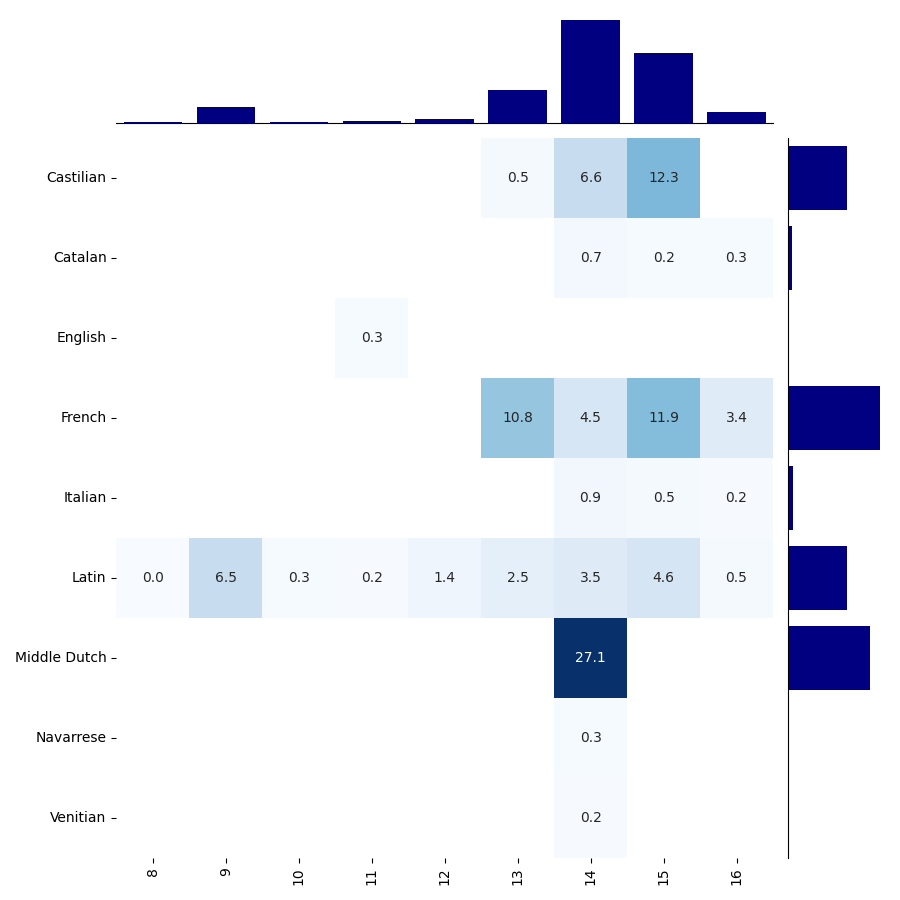
\includegraphics[width=\linewidth]{cv-for-ch/images/language.century.png}
      \end{subfigure}
      \hfill
      \begin{subfigure}[T]{0.40\textwidth}
        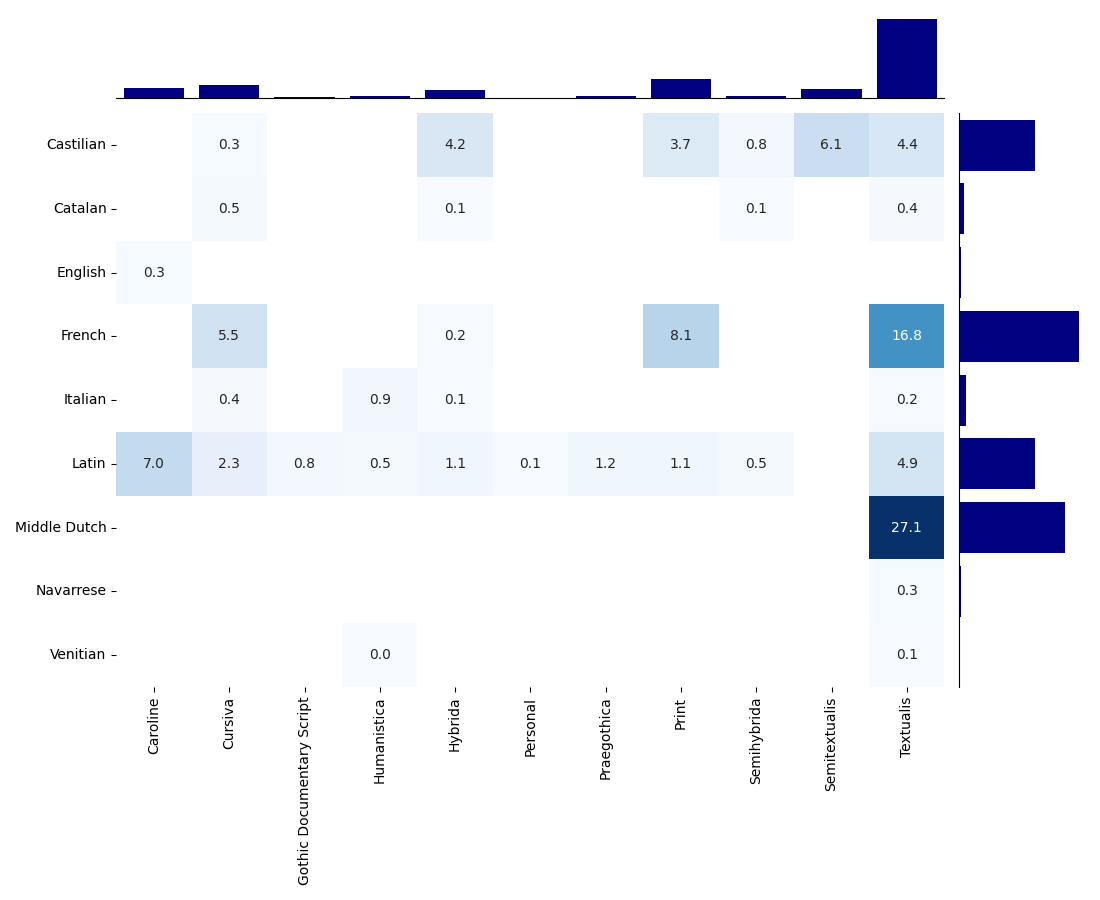
\includegraphics[width=\linewidth]{cv-for-ch/images/language.script.png}
      \end{subfigure}
      \caption{Distribution of the dataset across languages, centuries, and scripts, in \% of the total character count.}
      \label{fig:lang-cent-script}
    \end{figure}
    
\end{frame}

\begin{frame}{Fine-tuning}
    \begin{columns}
        \begin{column}{.5\linewidth}
            \begin{itemize}
                \item 20 manuscripts
                \item 10 epochs (each line seen ten times at most)
                \item Doable on a modern laptop in $\leq 10$ minutes ($\nearrow$ accessibility, $\searrow$ power consumption)
                \item 50 \% of their lines for training the model, 50 \% to test
                
            \end{itemize}
        \end{column}
        \begin{column}{.5\linewidth}
            \centering
            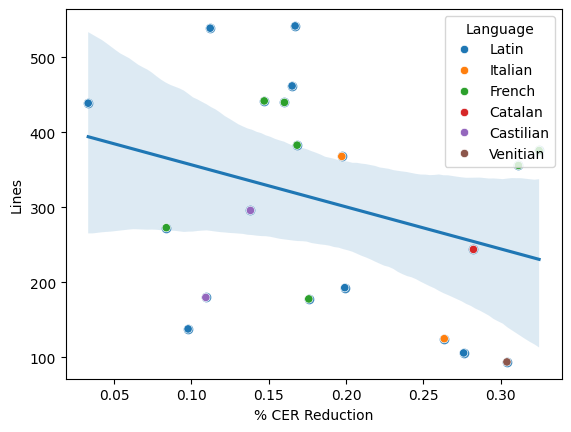
\includegraphics[width=\linewidth]{cv-for-ch/images/finetuning.png}
        \end{column}
    \end{columns}
\end{frame}

\begin{frame}{Generic yet specialized ?}
    \fullcite{kiessling:hal-04704547}
\end{frame}

\end{document}